% Going off the Thesis guidelines available here: http://www.lboro.ac.uk/students/welcome/research/codes-of-practice/appendices/
% A4 paper size selected, default is 11pt font, to change to 12pt use [a4paper, 12pt] as option to documentclass
\documentclass[a4paper]{report}

% Some useful packages for including images, colored font, etc.
\usepackage[dvips]{graphicx}
\graphicspath{{Figures/}}

\makeatletter
\def\maxwidth{\ifdim\Gin@nat@width>\linewidth\linewidth\else\Gin@nat@width\fi}
\def\maxheight{\ifdim\Gin@nat@height>\textheight\textheight\else\Gin@nat@height\fi}
\makeatother
\setkeys{Gin}{width=\maxwidth,height=\maxheight,keepaspectratio}
\usepackage{amssymb,amsmath}
\usepackage{longtable}
\usepackage{booktabs}

\usepackage{listings}
\usepackage{xcolor}
 
\definecolor{codegreen}{rgb}{0,0.6,0}
\definecolor{codegray}{rgb}{0.5,0.5,0.5}
\definecolor{codepurple}{rgb}{0.58,0,0.82}
\definecolor{backcolour}{rgb}{0.95,0.95,0.92}
 
\lstdefinestyle{mystyle}{
    backgroundcolor=\color{backcolour},   
    commentstyle=\color{codegreen},
    keywordstyle=\color{magenta},
    numberstyle=\tiny\color{codegray},
    stringstyle=\color{codepurple},
    basicstyle=\ttfamily\footnotesize,
    breakatwhitespace=false,         
    breaklines=true,                 
    captionpos=b,                    
    keepspaces=true,                 
    numbers=left,                    
    numbersep=5pt,                  
    showspaces=false,                
    showstringspaces=false,
    showtabs=false,                  
    tabsize=2
}
 
\lstset{style=mystyle}

\usepackage[numbers]{natbib}

\usepackage{color}
\usepackage{url}
% Used for subfigures
\usepackage{subcaption}
% Used for landscape pages
\usepackage{pdflscape}
% Used for hyper-links in contents, etc.
\usepackage[hidelinks]{hyperref}
\hypersetup{
    linktoc=all
}

% Global bibliography style
\bibliographystyle{plain}

% Set margins in all document to 3.5cm as per guidelines for binding
\usepackage[includeheadfoot,margin=3.5cm]{geometry}

% Used to including pdf files within pages
% use [draft] as option to output empty spaces rather than rendering all pages (useful when including lots of pdfs)
\usepackage{pdfpages}

% Used to produce headers and footers
\usepackage{fancyhdr}
\pagestyle{fancyplain}

% Used for removing title in bibliography sections
\usepackage{titlesec}

% Used to generate lists of abbreviations
\usepackage{nomencl}
\makenomenclature 
\renewcommand{\nomname}{List of Abbreviations} 

% To have a separate bibliography per Chapter uncomment this line
% See Introduction/Introduction.tex for example how to include the bibliography
%\usepackage{chapterbib}

% Line spacing defined at 1 and a half. I know it says 1.3 but its 1 and a half.
\linespread{1.3}

% Setup headers and footers
\fancyhf{}
\lhead{\leftmark}
% Center on all pages
% \fancyhead[C]{---Draft---}
% Page number placed on right side on odd pages and left side on even pages
\fancyfoot[RO, LE] {\thepage}


\begin{document}

% Give \subsubsection numbers
\setcounter{secnumdepth}{4}

% Title, Author, Abstract, Acknowledgement, Table of Content, List of Figures, List of Tables and List of Abbreviations
% Front matter of the Thesis
% Title page
% Loughborough University Thesis Access Form
% Loughborough University Certificate of Originality
% Abstract
% Acknowledgements
\title{\bf An Ad Hoc Wireless Sensor Network}

\author{by\\
Zhihao DAI\\
Sheng GAO\\
David WU\\
Keli ZHANG\\
Changrong CHEN\\
\\
{\bf COP531 Wireless Networks}\\
{\bf Coursework Report}\\
\\
Loughborough University\\
\\
\copyright
\hspace{1 dd} Group Three, 2020\\
\\
Feb. 2020
}
\date{} % Used to remove date from title so it can be set at any date rather than the current date

\maketitle

% Set page numbers to roman numerals for front matter
\pagenumbering{roman}

% % PDF exports of Word Documents available (Exported August 2012)
% % Thesis Access Form
% 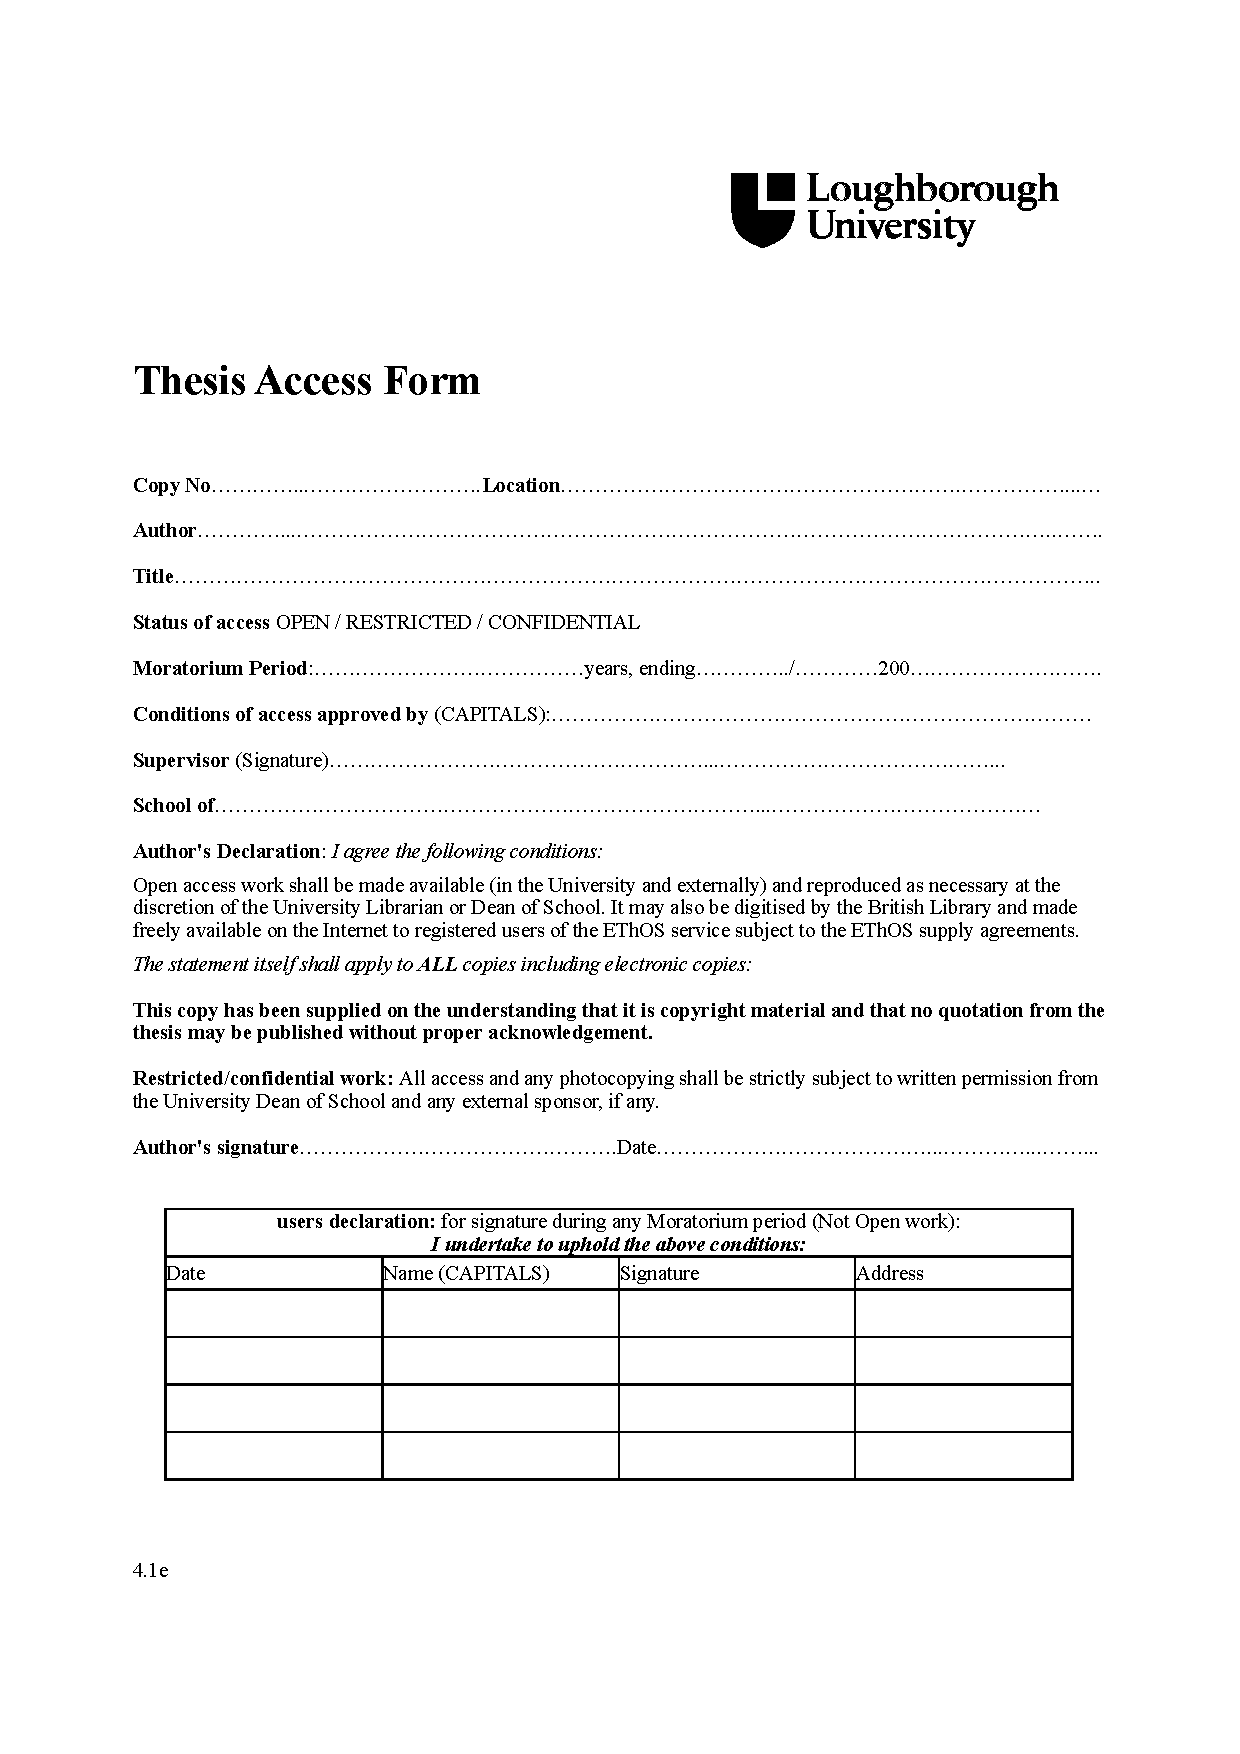
\includepdf[pages=1, pagecommand=, templatesize={5in}{10in}]{Front/LU/access.pdf}
% % Certificate of Originality
% 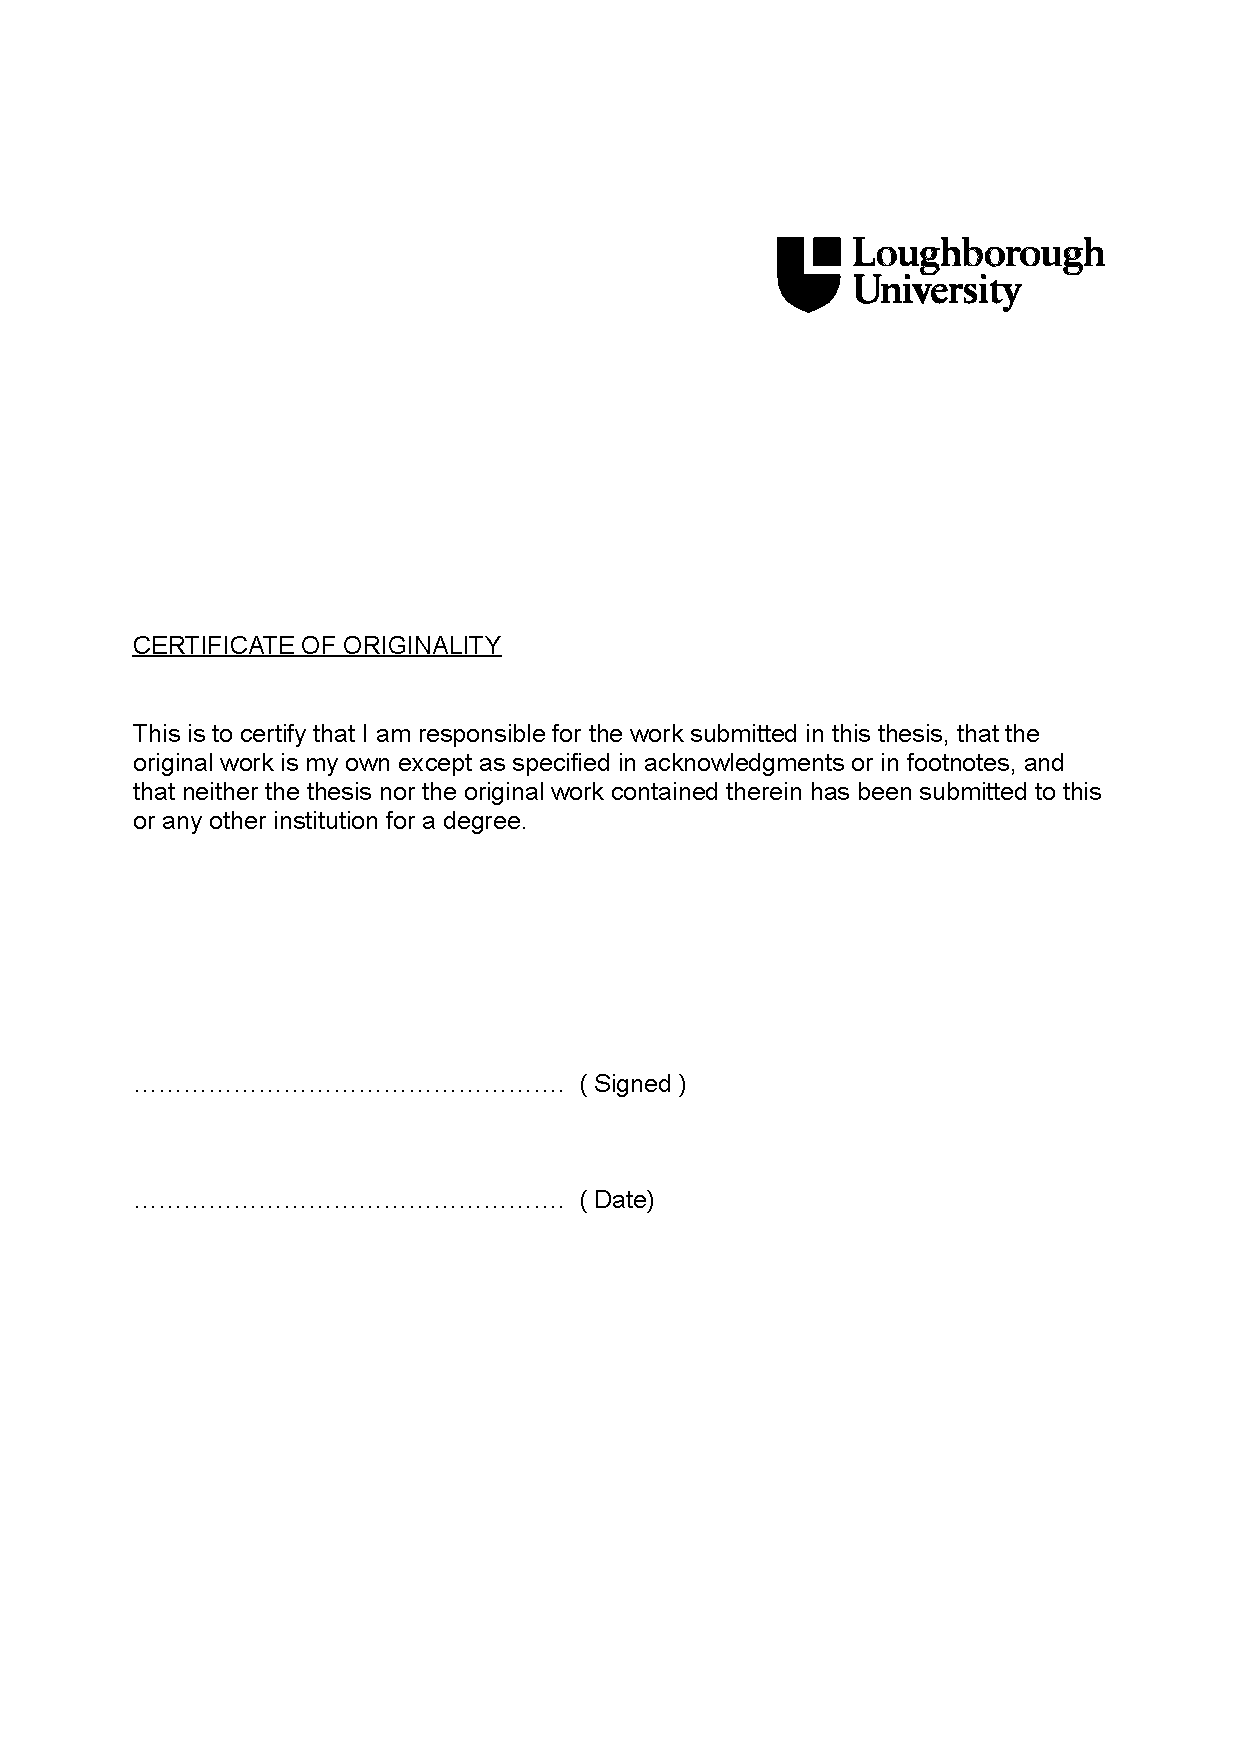
\includepdf[pages=-, pagecommand=, templatesize={5in}{10in}]{Front/LU/origin.pdf}

% Abstract
\addcontentsline{toc}{chapter}{Abstract}
\chapter*{Abstract}
In this report, we build a simple ad hoc wirelss sensor network composed of six Sensinode devices.
Among them one is designated as the source device, one is the destination device and others are intermediate devices.
The source device learns a route to the destination device from a simplified version of Ad Hoc On-Demand Distance Vector (AODV) routing protocol.
The route to the destination device could be either directly or through intermediate devices.
The source device sends a packet containing sensor readings to the destination regularly and expects an acknowledgement from the destination.
We conclude that we have successfully achieved all the required functions.
The proposed implement method of our algorithm worked very well and stable in the laboratory environment.

% % Acknowledgements
% \addcontentsline{toc}{chapter}{Acknowledgements}
% \chapter*{Acknowledgements}
% Acknowledgement section.

% Set the depth for your table of content
% Currently set at 2 (Chapter, Section, Subsection)
\setcounter{tocdepth}{2}
% Include a table of content
\tableofcontents

% Include a list of figures
\addcontentsline{toc}{chapter}{List of Figures}
\listoffigures

% Include a list of tables
% \addcontentsline{toc}{chapter}{List of Tables}
% \listoftables

% Include a list of Listings
% \addcontentsline{toc}{chapter}{List of Listings}
% \renewcommand*{\lstlistlistingname}{List of Listings}
% \lstlistoflistings

% Include a list of abbreviations using nomenclature package
%\addcontentsline{toc}{chapter}{List of Abbreviations}
%\printnomenclature[3cm] 

\newpage

% Set page numbering to arabic for body of Thesis
\pagenumbering{arabic}


% To keep everything neat I included each chapter as a separate .tex file
% Each contains a single chapter, they include all the settings defined in this .tex file
% Allows easier moving around of chapters

% Use \include{<path to .tex file>} to include documents
% For example
\chapter{Introduction}
\label{chap:introduction}


\section{Ad Hoc Wireless Sensor Network}

Ad Hoc Wireless Sensor Network is a type of network that has multiple hops, in-centralised, self-organizing wireless network; it also known as Multi-hop network, or Infrastructure-less Network, Self-organizing Network.

The entire network has no fixed infrastructure, each node has functional mobility, and they can stay in contact with each other dynamically in any way. In this kind of network, because the wireless terminal coverage has a restricted value range, two user terminals that do not communicate can use each other the forward packets directly. Growing node also has a router that can detect and maintain pathways to other nodes.

\subsection{Features of Ad Hoc Wireless Sensor Network}

\subsubsection{Independence}
The most significant distinction between ad hoc network and traditional communication network is, without the help of hardware infrastructure, that it could be able to build a mobile communication network at any place in any time. 
Its establishment does not depend on existing network communication facilities; It also has absolute independence.
This ad hoc network functionality is very well-suited to disaster relief, remote and other applications.

\subsubsection{Infrastructures}
Mobile hosts in ad hoc networks could travel around the network at will. Host movement can result in increasing or disappearing linkages between hosts, and the relationship between hosts will continuously change. The host may be a router in an ad hoc network; Therefore, motions allows the topology of the network to change constantly, in variable ways and at unpredictable speeds. The network topology is relatively stable for modern networks.

\subsubsection{Communication bandwidth}
There is no wired infrastructure in ad hoc networks, so wireless communication is used to communicate between hosts. The network bandwidth they provide is much smaller than that of wired channels, due to the physical features of wireless networks. However, given the collision, signal attenuation, noise interference and other factors produced by the competing Shared Wireless channel, the actual bandwidth available to the mobile terminal are far below the theoretical maximum bandwidth value.

\subsubsection{Energy}
The host is a mobile device that is ad hoc networks, such as a a portable computer, or a handheld computer. ad hoc network has the characteristic of limited energy because the host may be in the state of constant movement and the battery mainly provides the energy of the host.

\subsubsection{Distribution}
There is no central control node in an ad hoc network, and the hosts are connected via the distributed protocol. When one or some network nodes fail, the rest of the nodes may still function normally.


\section{Ad Hoc On-Demand Distance Vector (AODV) Routing Protocol}

AODV Routing Protocol \citep{rfc3561} is a reactive routing protocol commonly used for mobile Ad-Hoc Networks (MANETs), which is developed and implemented in Linux Operating System.
As implied in the name, the protocol is only initiated  when a data packet is needed to be sent to another node and no route is available at the moment.

A simplified version of AODV protocol is described as follows and can be divided into two stages, Route Request and Route Reply.

\subsection{Route Request}

The source node broadcasts a route discovery request (RREQ) to its neighbours.
Each neighbour except the destination, on receiving the RREQ, updates its own route table and rebroadcasts the RREQ.

\subsection{Route Reply}

The destination, on receiving the RREQ, updates its own route table and sends a reply (RREP) back to the source, through the route learned in the request stage.
Each neighbour except the source, on receiving the RREP, updates its own route table and forwards the RREP.
The source, on receiving the RREP, updates its own route table and thus learns a route to the destination.

\section{Task}

In this report, we attempt to build a Ad Hoc Wireless Sensor Network, with AODV as the routing protocol.
The full details of our version of AODV protocol are described in Section \ref{sec:design-aodv}.

The network is composed of six Sensinode devices, among which one is the source sensing device, one is the destination sensing device and the others are intermediate nodes.

The source sends out sensor readings regularly to the destination using the route learnt from AODV protocol, which goes through intermediate nodes.

To cope with the dynamic changes in the network, acknowledgements for data delivery are introduced.
The destination device, on receiving the sensor readings, sends back an acknowledgements to the source.
When the source doesn't receive an acknowledgement for a previous data packet, it should consider the previous route lose and initiate AODV protocol to learn a new route.



\chapter{Network Design}
\label{chap:design}

\section{Assumptions}

Several assumptions are made in designing the network.
\begin{enumerate}
    \item There is only one source device and one destination device in the network. All other nodes are intermediate nodes.
    \item The address of the destination device is fixed.
    \item All links between neighbouring nodes are bi-directional. If a node is able to send a packet directly to a neighbour, it should be able to receive a packet directly from the neighbour.
\end{enumerate}

\section{Network Components}

\subsection{Sensinode Devices}

In this coursework, the physical node we are using is called ‘Sensinode’, which is invented and created by Sensinode Ltd, a company that focuses research on the Internet of Things(IoT). 
Sensinode’s solution enables development and support of device networks built around the IPv6 protocol and Embedded Web Services. 
The Sensinode NanoService provides end-to-end web services optimized for the constraints of M2M deployments. 

Sensinode is running on Contiki Operating System \footnote{http://www.contiki-os.org}, which provides a variety of handy and primitive APIs for building Wireless Sensor Network.
Applications running on Contiki OS are written in C programming language.

\subsection{Person Computers}
Sensinode devices in the network are connected to person computers for downloading the program and displaying the output. Although those computers are not part of the network, they play an important rule in understanding the flow of information inside the network.


\section{Roles Inside Network}
\label{sec:architecture}
There are three different roles inside the network--the Source Device, Intermediate Devices as well as the Destination Device.

\subsection{Source Device}
Source device in the routing discovery stage is as a first originator for broadcasting request message (RREQ) to other nodes, connecting other intermediate nodes to find destination node in Ad-Hoc wireless sensor network. After receiving a Reply message (RREP) from the destination node, it reads all the routing information such as route index and choose the best route to send packets. At the packet delivery stage, it is able to collect all information such as light, temperature, voltage and sent them in a single packet to the destination node through intermediate nodes. Type of data to transfer is also able to change by clicking the desired button on the source node.

\subsection{Intermediate Devices}
There are four intermediate nodes in our desired Ad-Hoc wireless sensor network. At route discovery stage, their job is receiving a broadcast from the originator and broadcast those request message (RREQ) again to other intermediate nodes until it reached destination nodes. In contrast, it will create a reverse path to carrying reply message (RREP) from destination node to source node.

\subsection{Destination Device}
The destination device is the opposite side of the originator, it works with other nodes to establish a route which works most efficient. At routing discovery stage its job is to receive the RREQ and check if itself is the destination node; if destination node confirmed it would send the RREP back to where the RREQ comes from. At the packet delivery stage, its job is receiving the packet of different readings such as temperature, light, voltage and eventually display all information that source node gathered on the screen of computers.

\section{Stage One: Route Discovery}
\label{sec:design-aodv}
Our design of route discovery is a simplified version of AODV protocol. There are two sub-stages inside route discovery--Route Request and Route Reply.

\subsection{Route Request}

When the source device needs to send a data packet to the destination and no route towards the destination is found inside its route table, the source device initiates the AODV protocol.
The source broadcasts a route discovery request (RREQ) to its neighbours, which contains a One Byte Unique Header Field, RREQ ID, and destination address.
The RREQ ID inside the packet increments by one each time a new RREQ is sent.

\begin{figure}
\centering
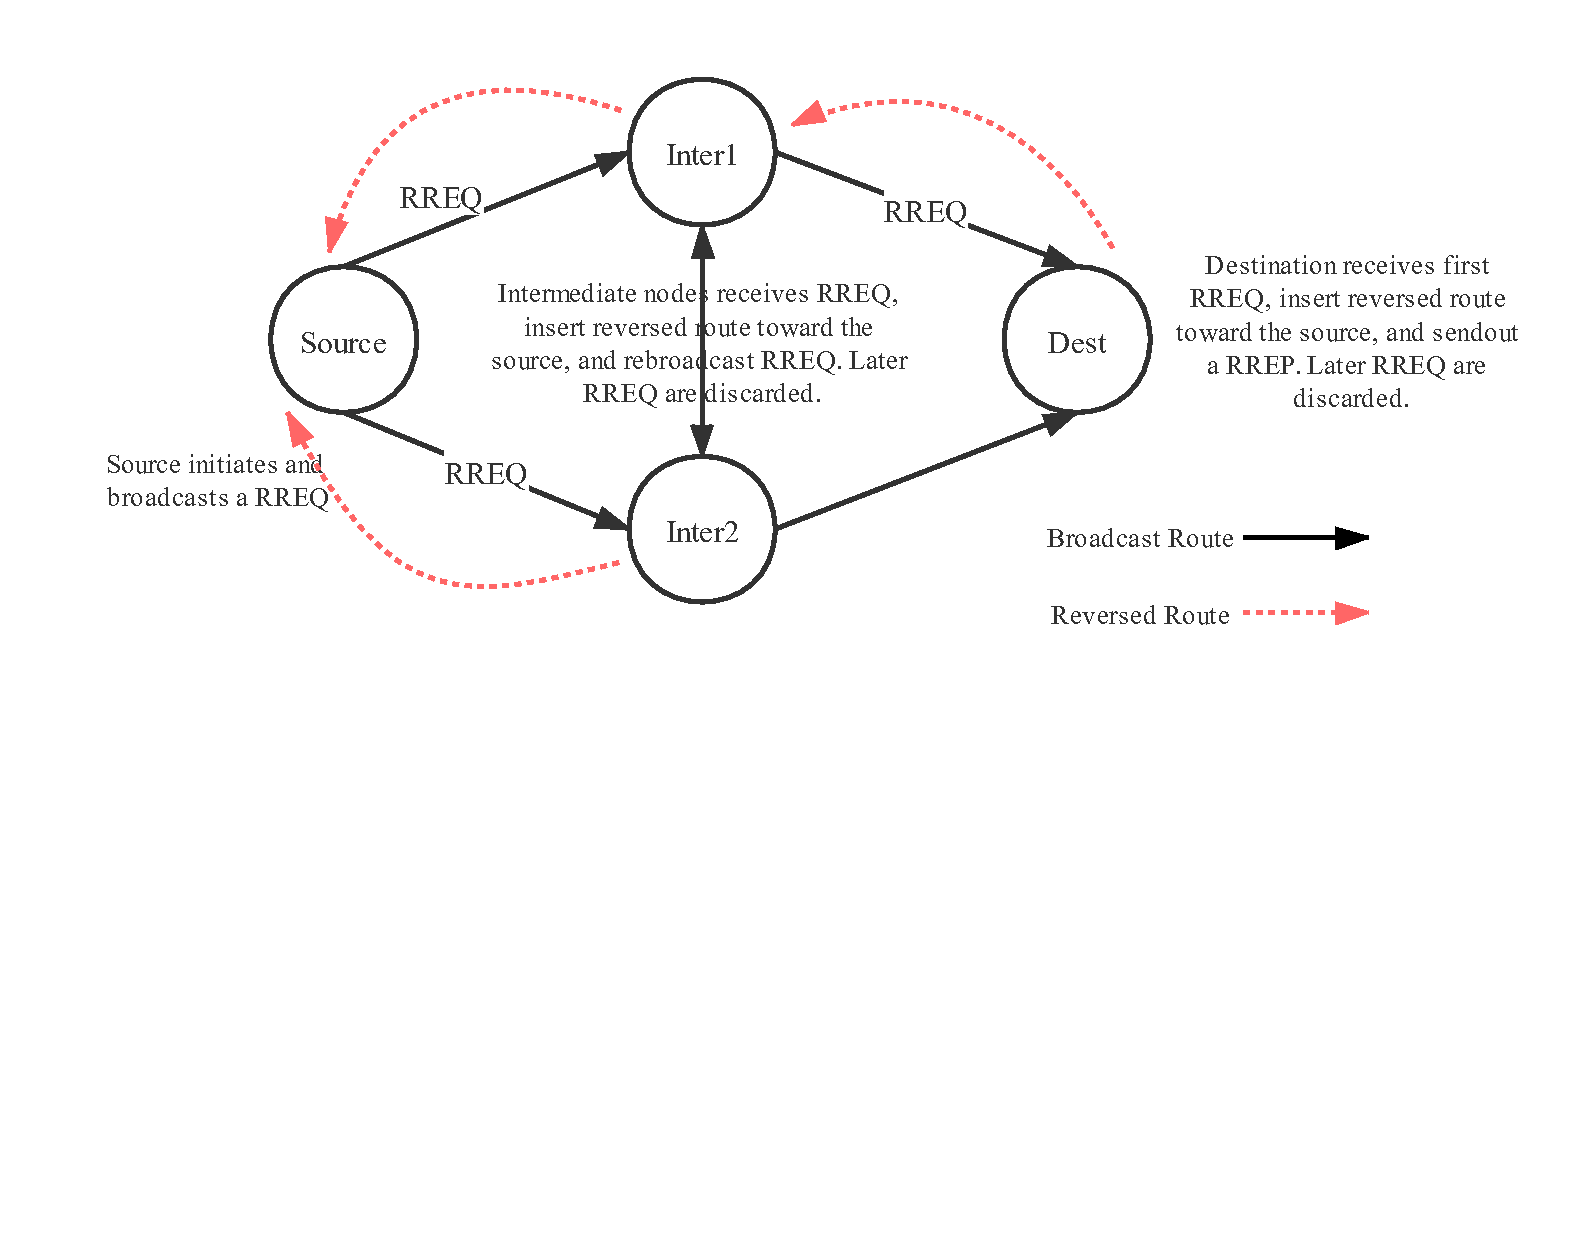
\includegraphics[width=\textwidth]{request}
\caption{Broadcasting a Request (RREQ) in AODV Protocol.}
\label{fig:request}
\end{figure}

Each intermediate node, on receiving the first RREQ, verifies the Unique Header Field, whose value should be constant 0x33, to distinguish our group's packets from others'.
If the RREQ is verfied, the intermediate node inserts a reversed route into its route table. The destination of of the route is the source device and the next hop is the node it receives the RREQ from.
The node then re-broadcasts the RREQ to its neighbours.
The node saves the address of the source and the RREQ ID as the last source and RREQ ID it receives.
The node, on receiving later RREQs of the same source and RREQ ID, discards all late-coming RREQs.


The destination device, on receiving the RREQ, likewise, verifies the Unique Header Field and inserts a reversed route into its route table.
However, it doesn't re-broadcast the RREQ.
It sends a route discovery reply (RREP) towards the source device.
The destination device saves the address of the source and the RREQ ID as the last source and RREQ ID it receives.
The destination device, on receiving later RREQs of the same source and RREQ ID, discards all late-coming RREQs.



\subsection{Route Reply}
The RREP contains a Unique Header Field, the source (destination device) addres, the destination (the source device) address and the RSSI value of the RREQ packet the destination device receives (first\_rssi).
The destination device sends out RREP to the node it receives the RREQ packet from, essentially using the route learns from the RREP packet.

\begin{figure}
\centering
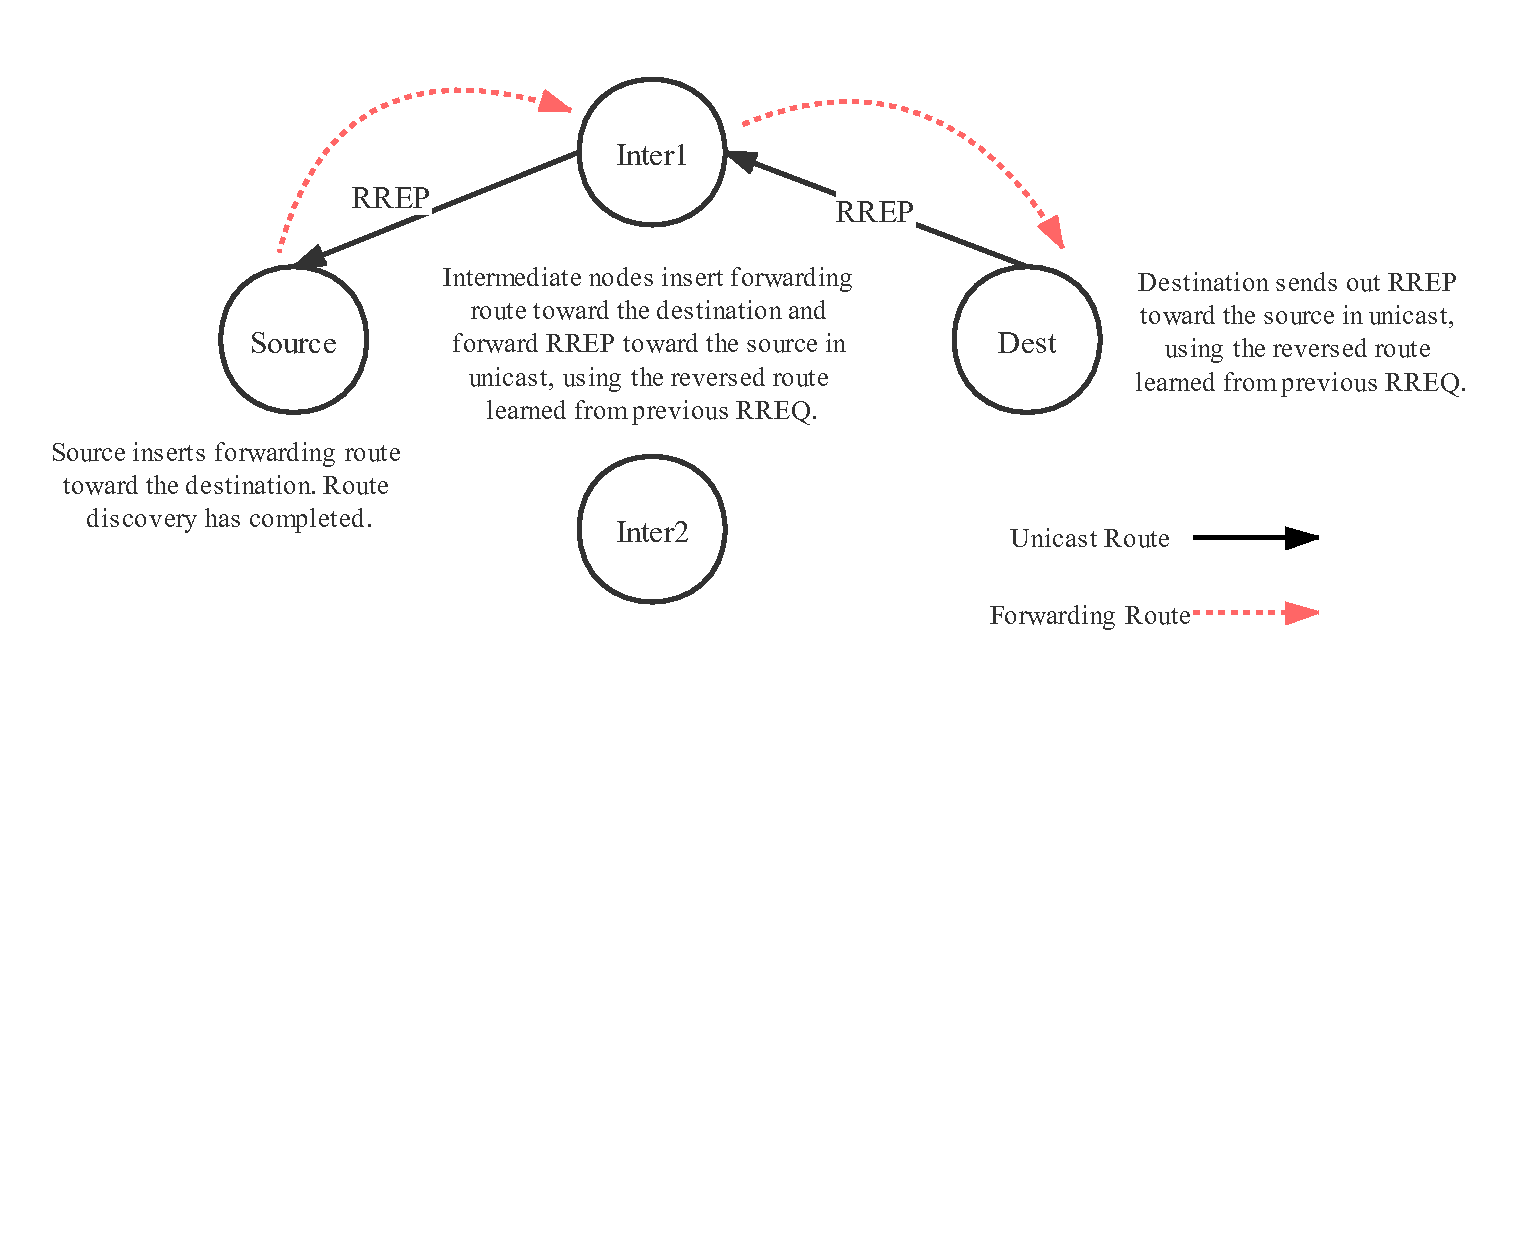
\includegraphics[width=\textwidth]{reply}
\caption{Forwarding a Reply (RREP) in AODV Protocol.}
\label{fig:request}
\end{figure}

Each node, on receiving the RREP, verifies the Unique Header Field, whose value should be a constant 0x33, to distinguish our group's packets from others'.
The node appends its address, battery level and RSSI value of the RREP packet it receives to the packet.
The node inserts a forwarding route towards the destination device into its own route table.
The destination of the route is the destination device and the next hop is the node it receives RREP from.
The route index is computed using the first\_rssi value and the appended information by previous nodes.
The node then forwards the RREP packet through the route is learns from the request stage.

The source node, on receiving the RREP, likewise, verifies the Unique Header Field, inserts a forwarding route into the route table and computes the route index.
However, it does not forwards RREP packet.
At this moment, the source node has learnt a new route towards the destination.

\subsection{Route Expiry and Renewal}
Each route learnt from AODV protocol, by default, has a lifetime of $10$ seconds.
However, if the route has been proven to be valid, the route will be renewed immediately by the node.
Concretely, if node A receives a packet from node B originated from node C, the route whose destination is node C and next hop is node B in node A's route table will be renewed right away.

If the route has been proven to be invalid, the route will be purged immediately by the node.
Concretely, if node A sends a data packet to node C through node B but doesn't receive an acknowledgement from node C, the route whose destination is node C and next hop is node B in node A's route table will be purged right away.

Route Expiry and Renewal ensures that each route is always up to date and forces the node to initiate a route discovery when a route is no longer valid.

\section{Stage Two: Data Delivery}

At this stage, for source node, it has its primary process, where every time it initiated, it will wait two seconds and then decide what type of value it is going to collect; Whether temperature/light value or battery voltage. Then it will send a packet to intermediate nodes ask them to forward to the destination node. Since it is multithreading, at packet received call-back, it will check if it is destination while a packet received. If the answer is negative, it will be looking up route table to see if destination in route table or not, it will unicast to next route entry if it finds destination in route table, or it will redo route discovery process if there is no destination in its route table. At the same time button even, handler is waiting to check which button has been clicked; If the button one has clicked the information output mode will be modified, whereas sensor value content will be modified while button two has been clicked.

As for the destination node, the job is receiving packets and displaying them on-screen of the PC. It has multi-thread as well. It will initialize event handler first, while it received a packet, it will check whether if itself is a destination. If the answer is positive, it will resolve what content that packet have, whether it is temperature/light value or battery value, and print everything on screen; if the answer is negative, it will be looking up in route table and check if it needs to unicast route entry or redo the route discovery. Simultaneously debug information handler will check if the button has pressed with button the event handler, if the button has been pressed, it will change debug output. 







\chapter{Implementation}
\label{chap:implementation}

\section{Sensors Reporting}

In this experiment, there are three kinds of sensors value that should be obtained by using Analog-to-digital converter (ADC), including temperature, light and battery voltage. 
In the Sensinode device, these sensors should be initialled based on the ADC before obtaining the values. The build-in function will be used as follow: \texttt{sensors\_find(ADC\_SENSOR)}. After initialling the sensors, the original value needed can be read directly. 

However, the true values are still needed to convert by using the specific formulas after using the function \texttt{sensor->value(ADC\_SENSOR\_TYPE\_TEMP)}. 

\subsection{Temperature Reporting}

For temperature sensor, the true value of temperature is the environmental temperature, which is got by using the Formula \ref{equ:temperature} as follow.

\begin{equation}
    Temperature = \frac{0.61065 \times ADC - 773}{2.45}
\label{equ:temperature}
\end{equation}

where the temperature is the true value after calculating and the ADC is the argument obtained before. 

\subsection{Light Reporting}

For light sensor, the illuminance obtained from the sensor in Sensinode device is between $40$ Lux and $600$ Lux. The original value can be got by using the function \\
\texttt{sensor->value(ADC\_SENSOR\_TYPE\_LIGHT)}. 
The specific Formula \ref{equ:illuminance} is shown as follows.

\begin{equation}
    Illuminance = 
    \frac{600 \times 1.25 \times ADC}{2047 \times 0.9}
\label{equ:illuminance}
\end{equation}
where the Illuminance value is the true value after calculating and the ADC is the same as the above.


\subsection{Battery Level Reporting}
Another sensor is the battery sensor, which gets the voltage of battery. The detailed formula \ref{equ:battery} is displayed as follow:

\begin{equation}
    Battery = 
    \frac{3 \times ADC \times VDD \times 3.75}{2 \times 2047 \times 2047}
\label{equ:battery}
\end{equation}

where the Battery is the true voltage after converting, the ADC and VDD mean that the working voltage inside the Sensinode device, which can be obtained from the sensor directly by the function \texttt{sensor->value(ADC\_SENSOR\_TYPE\_BATTERY)} and \\
\texttt{sensor->value(ADC\_SENSOR\_TYPE\_VDD)}.

\subsection{Button Events}
For every sensor, there are two buttons separately that can control two modes. One of them is to switch on/off sending data. Another one is to choose which value should be displayed. For the specific implementations, the listening event will be executed by using the build-in variables (\texttt{button\_1\_senso}, \texttt{button\_2\_sensor}, \texttt{sensor}). 

When the value of sensor is equal to \texttt{button\_1\_sensor}, it means that the button has been triggered. The button2 is likewise to the button1. After pressing the buttons, the value will change the current status, and become the opposite value. 

\section{Stage One: Route Discovery}

In this part, the AODV algorithm is implemented based on the route discovery in Rime library \citep{dunkels2007rime,dunkels2007adaptive} \footnote{http://contiki.sourceforge.net/docs/2.6/a01798.html}. 
It can mainly be divided into two parts, including route requests, route reply.

For route requests, the control packets will be sent to other nodes by using function \texttt{netflood()}. The detailed information in the control packet have destination address, request ID, pad, group number.

For route reply, the packets will be sent by the destination node after finding a path from source to destination. The reply data includes request ID, hops number, destination address, originator address, group number, request RSSI. In our algorithm, the RSSI plays a crucial role in route discovery.  

During route discovery, the route index will be calculated by the Formula \ref{equ:index} as follows.

\begin{equation}
    \text{Route Index} = 
    \frac{\sum_i^N{RSSI_i}}{N \times H}
\label{equ:index}
\end{equation}

where $RSSI_i$ is the $i$-th intermediate node RSSI level, $N$ is the number of the intermediate nodes and $H$ is the number of hops from the source node to the destination node on the route.  

Route Index as a main role in route discovery is quite important, which can find the current closest device based on the value in the whole network. 
After reaching the destination, the destination node will reply to the source node and then format an active path for sending data. After getting the route index, it will be used and forwarded by each node. 

\section{Stage Two: Data Delivery}

Before sending the headers and data, all value will be packed by using a \texttt{struct}, and then the build-in function (\texttt{multihop\_send()}) is used for transferring the data. When the destination node received the packets from the source node, the acknowledgement will return to the source node and make sure that the packets have been received.

% \section{Sensors Displaying}







\chapter{Test \& Analysis}
\label{chap:test}

This chapter is divided into 2 parts. 
The first part is for requirements testing, where experiments are conducted to evaluate whether all four requirements of the coursework have been successfully implemented.
The second part is for network performance testing, where experiments are conducted to evaluate the performance of the whole network.
In addition, the effects of data acknowledgements on the performance are analyzed.

\section{Requirements Testing}

For requirements testing, all 6 nodes are included. 
As detailed in Section \ref{sec:architecture}, one node acts as the source device, one as the destination device, and the others as intermediate nodes.

Figure \ref{fig:test-req} shows the position of all six nodes in the network. 
The source device is placed on the leftmost side, the destination device on the rightmost side, and the intermediate nodes in the middle.

\begin{figure}
\centering
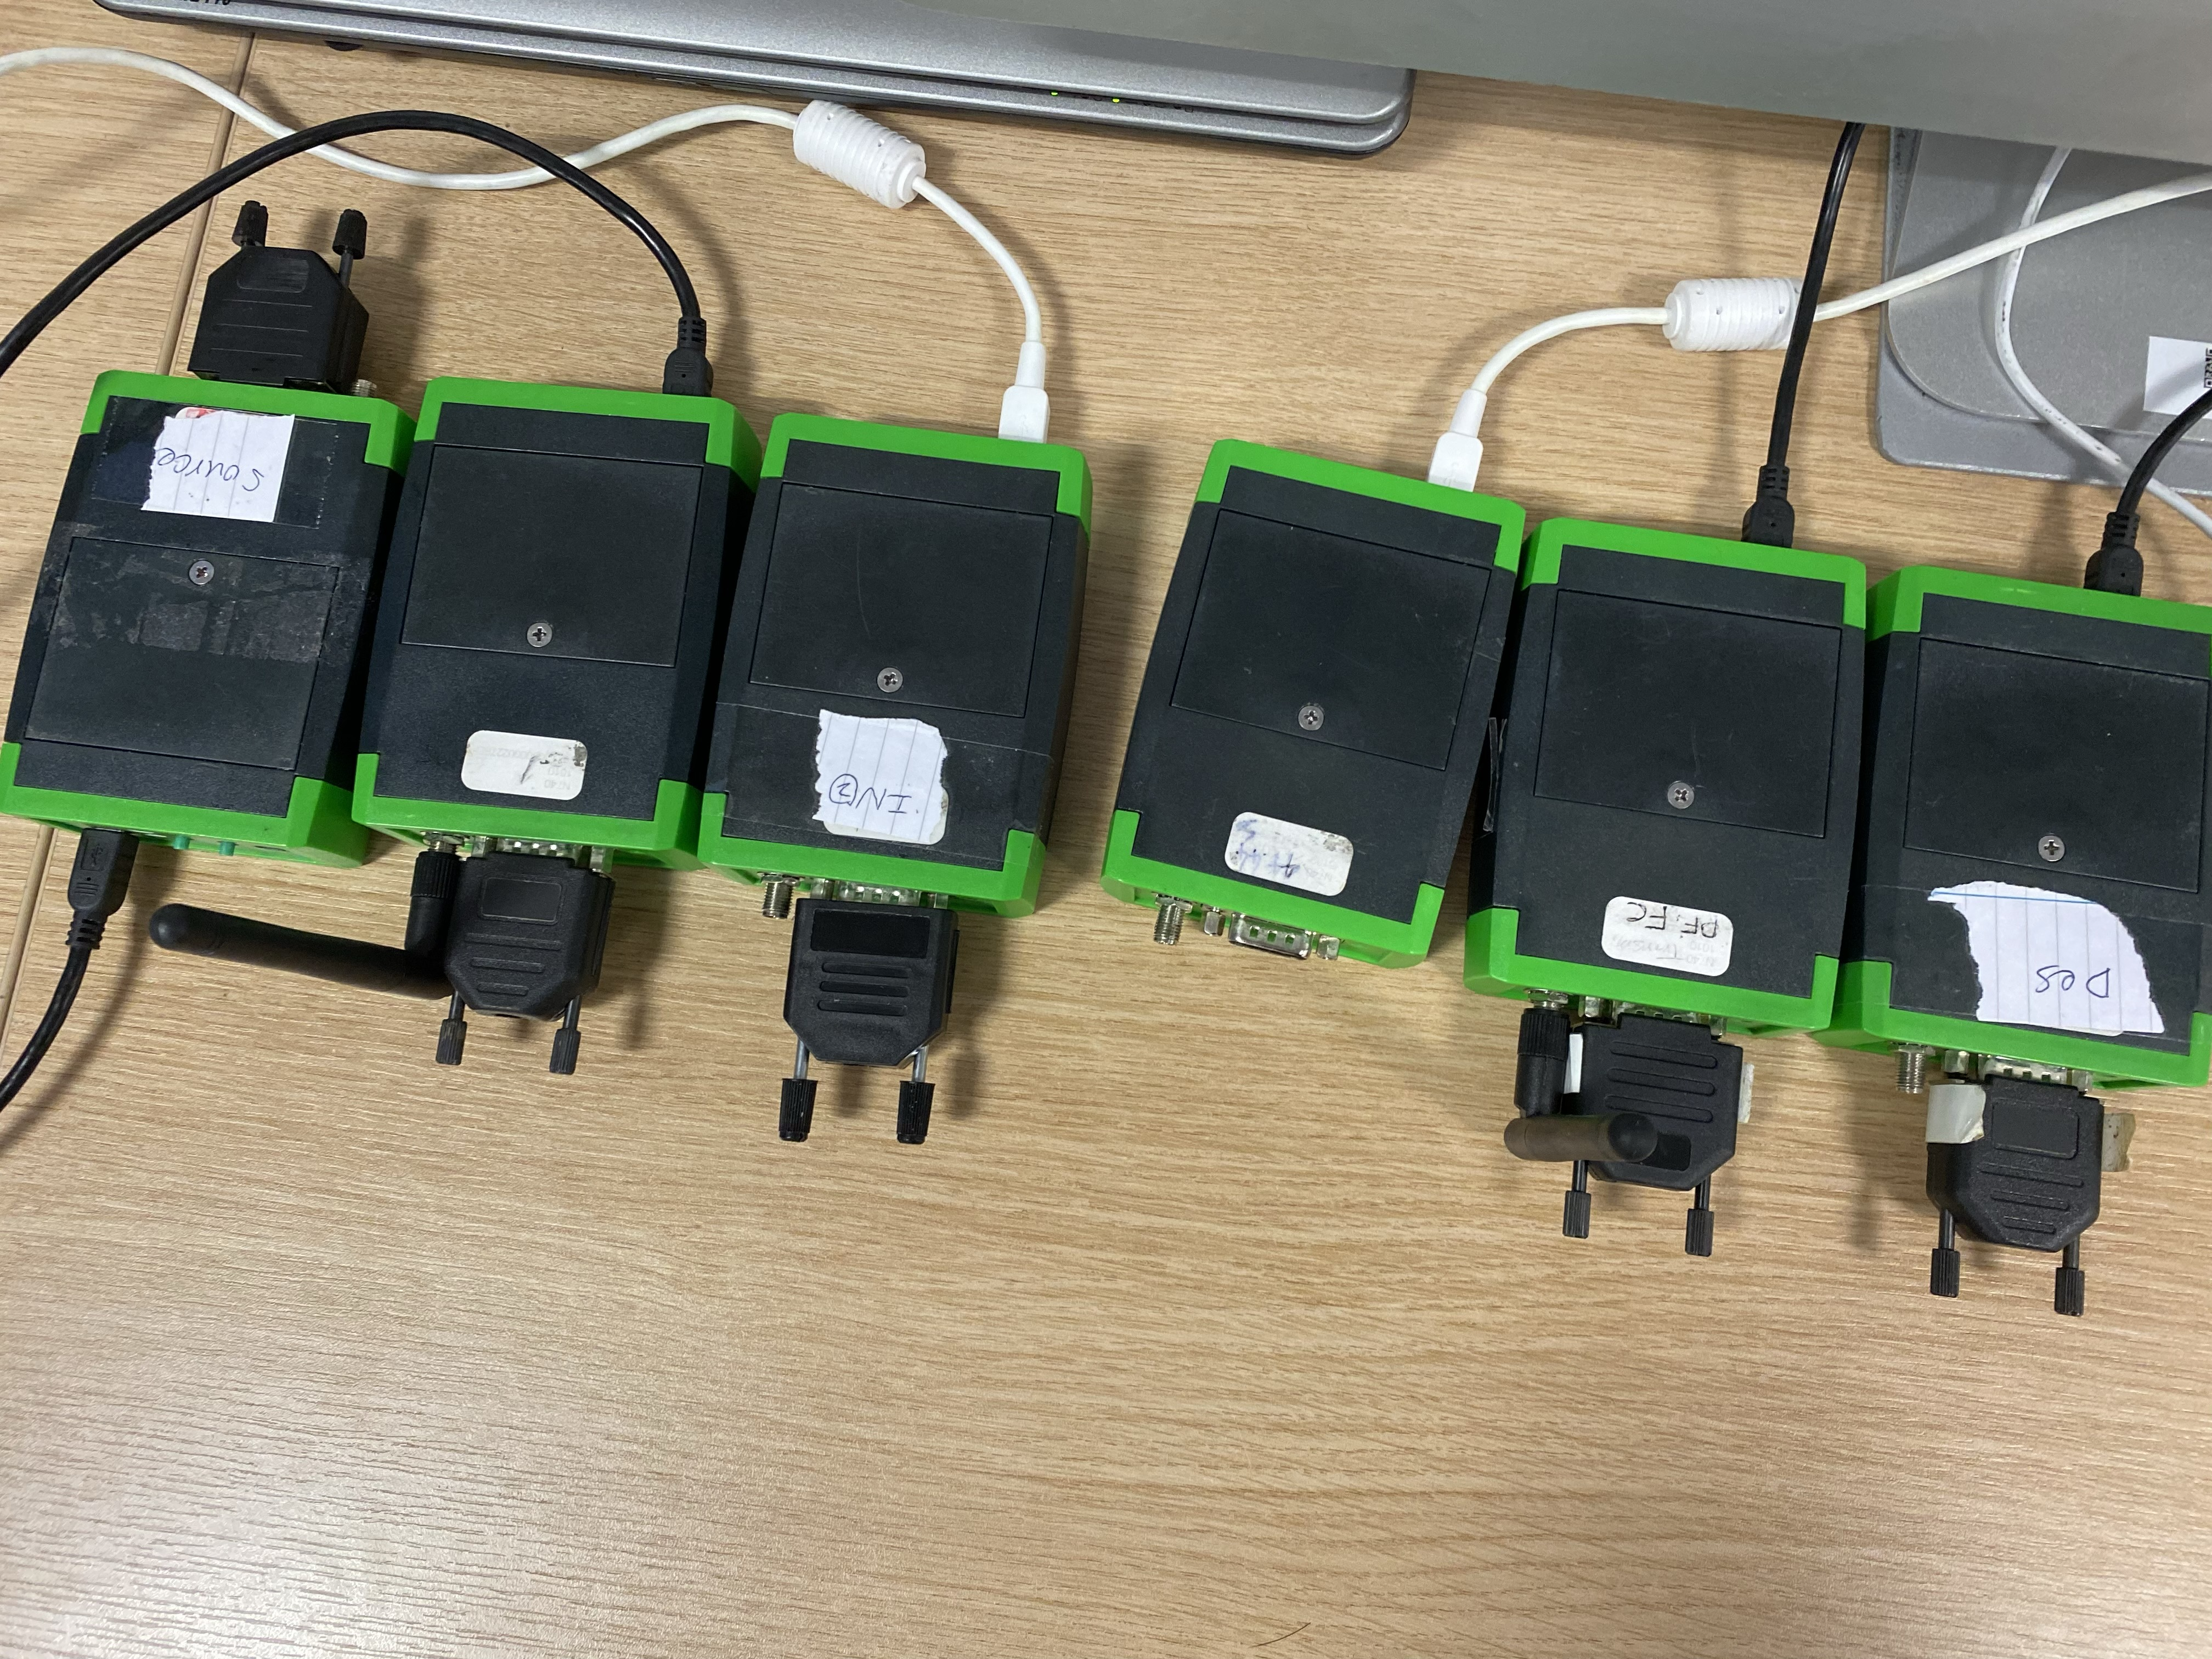
\includegraphics[width=0.7\textwidth]{test-req}
\caption{Position of All Six Nodes in the Network.}
\label{fig:test-req}
\end{figure}

Each node is assigned with a unique MAC address within the group. The source device is assigned with address of AA:AA (170:170), while the destination device is DF:DF (223:223).
The remaining intermediate nodes are assigned with addresses of 01:01, 02:02, 03:03 and 04:04 respectively.


\subsection{Requirement 1 \& 3: Regular Sensors and Route Reporting on Destination Node}

\subsubsection{Experiment Steps}

All devices are turned on. Button 1 on the source device is pressed to initiate regular sensors reporting.

\subsubsection{Expected Results}
The source device should first initiate a route discovery request (RREQ) towards the destination device.
Once it receives a route discovery reply (RREP) and inserts a route, it should send out a data packets using the learned route per 2 second.

If the learned route is valid, the destination device should receive the data packet and send back an acknowledgement.

If the learned route is invalid (eg. weak signal, changes of position), the destination device would not receive the data packet and not send back an acknowledgement.
In that case, the source device would not get an acknowledgement and should initiate a route discovery request again and stop sending out data packets until a new route is learned.

\subsubsection{Results}
Figure \ref{fig:test-1-source} shows the output from the source device.
Once the button is pressed, the source device initiates a route discovery request towards 223.223, which is the destination device.
A reply is received directly from the destination and a new route is thus learned, of which the route index is $-78.0$.

\begin{figure}
\centering
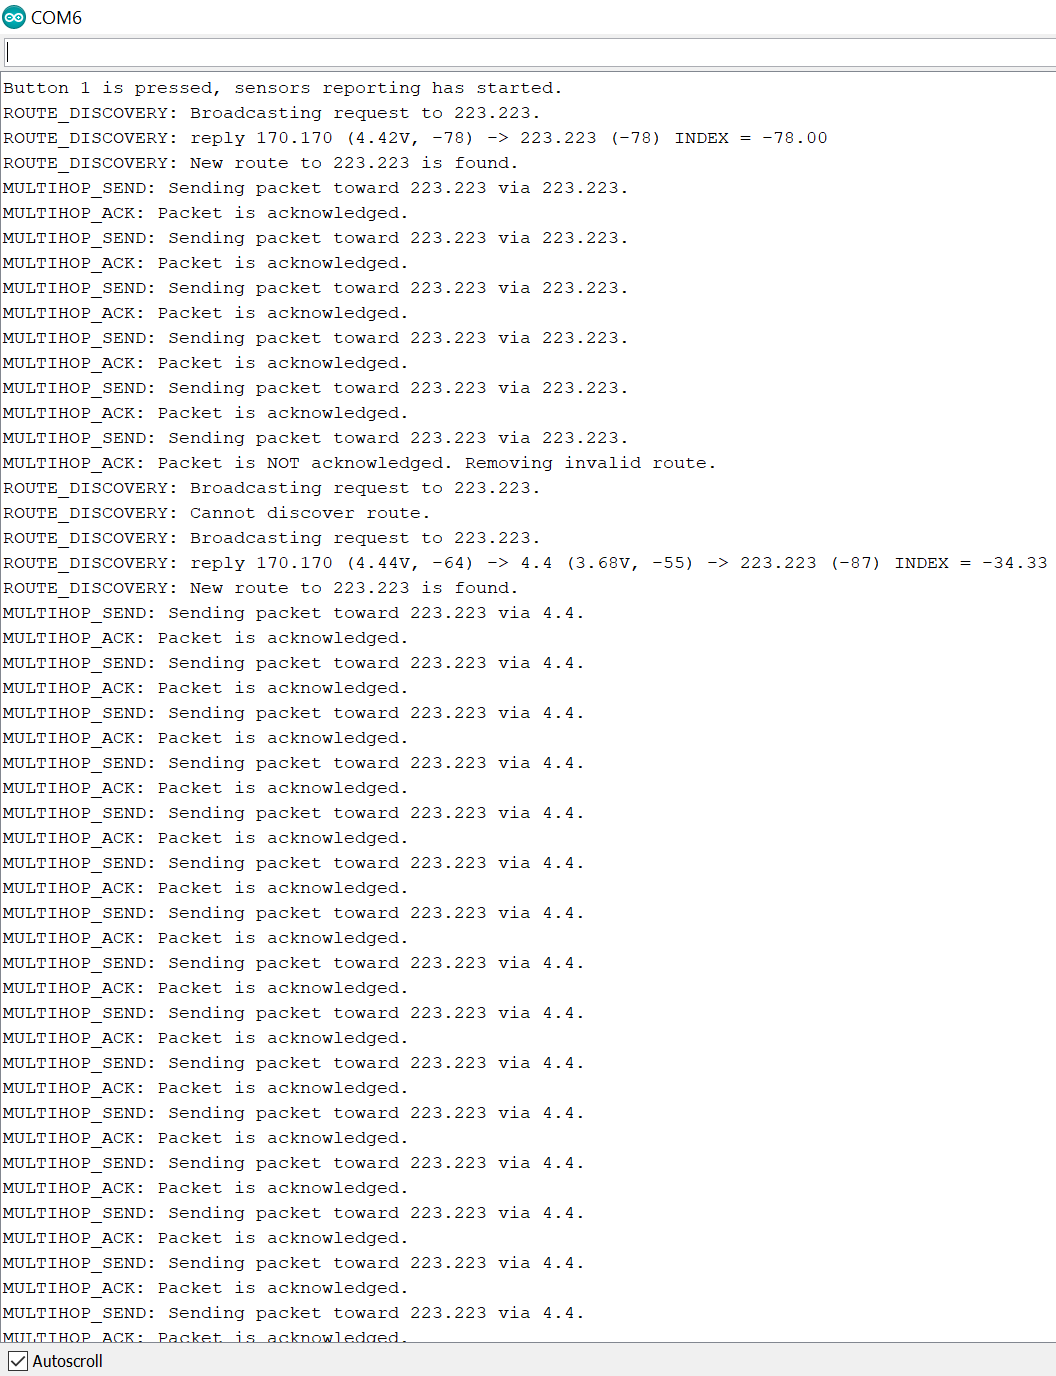
\includegraphics[width=0.7\textwidth]{test-1-source}
\caption{Output from the Source Device After Regular Sensors Reporting Is Started.}
\label{fig:test-1-source}
\end{figure}

The source device starts sending out sensors reading regularly towards the destination device through the route.

On the sixth data packet, an acknowledgement is not received. The source perceives that the route is no longer valid and initiates a route discovery request towards 223.223 again.
A reply is later received from 4:4, which is the fourth intermediate node, and a new route towards the destination is thus learned, of which the route index is $-34.33$.

The source device starts sending out sensors reading regularly towards the destination device through the route again.

Figure \ref{fig:test-1-dest} shows the output from the destination device.
The destination device first receives route discovery request (RREQ) from 170:170, which is the source device and sends back an reply (RREP).
It later receives and displays six data packets from the source, all of which include temperature and battery reading from the source device.
In addition, the data packets include the route each packet take from the source to the destination.

\begin{figure}
\centering
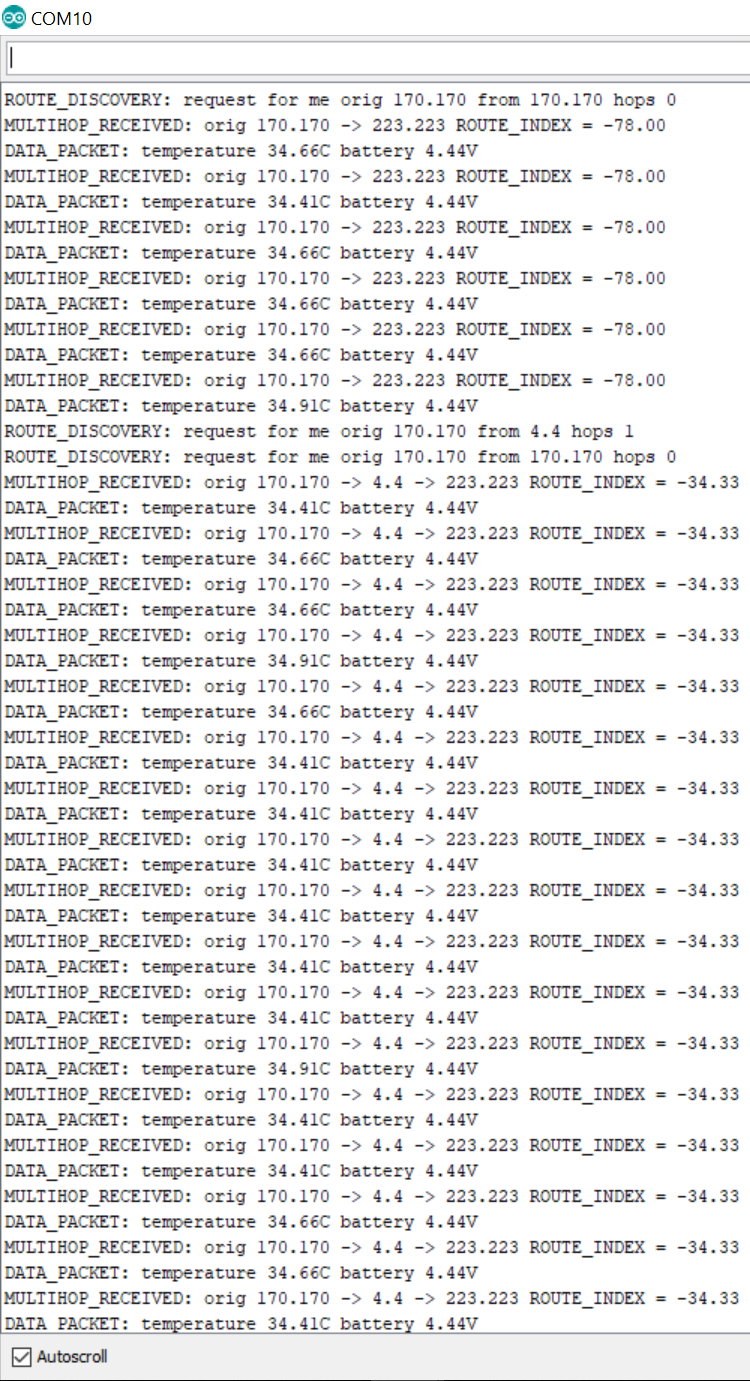
\includegraphics[width=0.7\textwidth]{test-1-dest}
\caption{Output from the Destination Device After  Regular Sensors Reporting Is Started.}
\label{fig:test-1-dest}
\end{figure}

Two new RREQ are then received since the source perceives that the previous direct route is no longer valid and initiates new route discovery requests.
After the new route through 4:4 is established, the destination device starts receiving data packets from the source again.


\subsection{Requirement 2: On-Demand Sensors Switching on Source Node}

\subsubsection{Experiment Steps}
All devices are turned on. 
Button 1 on the source device is pressed to initiate regular sensors reporting.
After a while, Button 2 on the source device is pressed to switch from temperature reporting to light reporting.

\subsubsection{Expected Results}
Once Button 2 is pressed, the source device should switch from temperature reporting to light reporting, or from light reporting to temperature reporting.



\subsubsection{Results}

Figure \ref{fig:test-2-source} shows the output from the source device.
The source device first sends out data packets towards the destination (223:223) through the fourth intermediate node (4:4).
The source device, on receiving that Button 2 is pressed, switches to reporting light sensors reading. 

\begin{figure}
\centering
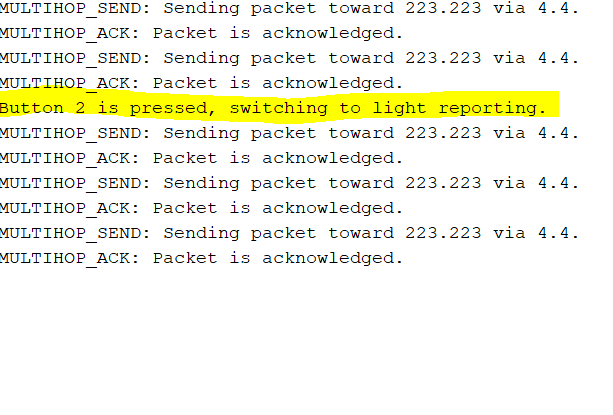
\includegraphics[width=0.7\textwidth]{test-2-source}
\caption{Output from the Source Device After Sensors Reporting Is Switched.}
\label{fig:test-2-source}
\end{figure}

Figure \ref{fig:test-2-dest} shows the output from the destination device.
The destination device first receives data packets that contain temperature and battery voltage readings.
After Button 2 on the source device is pressed, it starts receiving data packets that contain light and battery voltage readings.

\begin{figure}
\centering
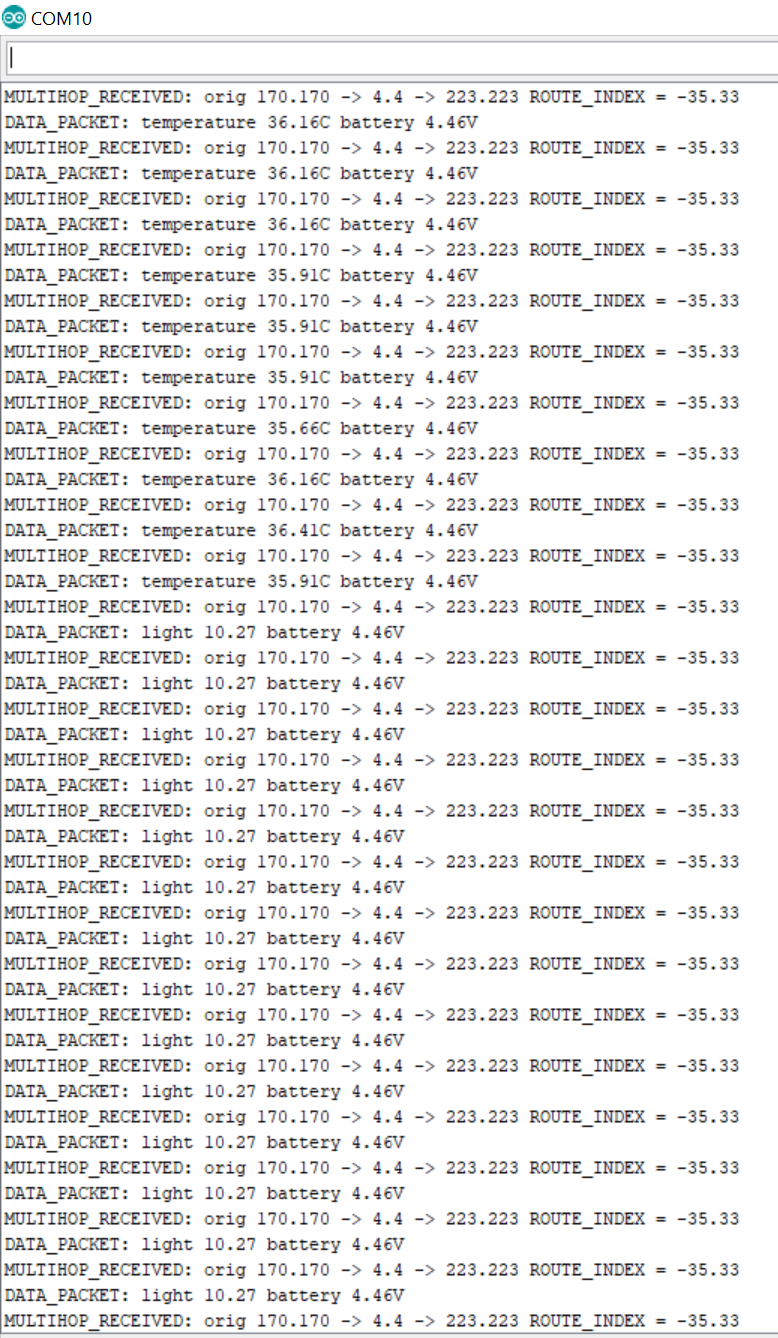
\includegraphics[width=0.7\textwidth]{test-2-dest}
\caption{Output from the Destination Device After Sensors Reporting Is Switched.}
\label{fig:test-2-dest}
\end{figure}

\subsection{Requirement 4: Dynamic Routing}

In this test, sudden changes of intermediate nodes are introduced in the middle of the data delivery by switching off some of intermediate nodes.
According the requirement, one should expect that the source device learns of the lost of intermediate nodes and learns a new route right away.

\subsubsection{Experiment Steps}
All devices are turned on.
Button 1 on the source device is pressed to initiate regular sensors reporting.
After a stable non-direct route is established between the source and the destination, one of the intermediate nodes on the route is switched off.

\subsubsection{Expected Results}
After one of the intermediate nodes on the route is switched off, the source device will no longer be able to send data packets to the destination using the previously learned route.
It receives no acknowledgement from the destination and should then perceive that the route is no longer valid.
The source is expected to initiate a new route discovery request (RREQ) to learn a new route.

\subsubsection{Results}

Figure \ref{fig:test-4-source} shows the output from the source device.
At first, the source device learns a route towards the destination through the fourth intermediate node (4:4).
After the fourth intermediate node is switched off manually, the source device receives no acknowledgement for the last data packet it sends.
It removes the route from its route table and initiates a new route request towards the destination.

\begin{figure}
\centering
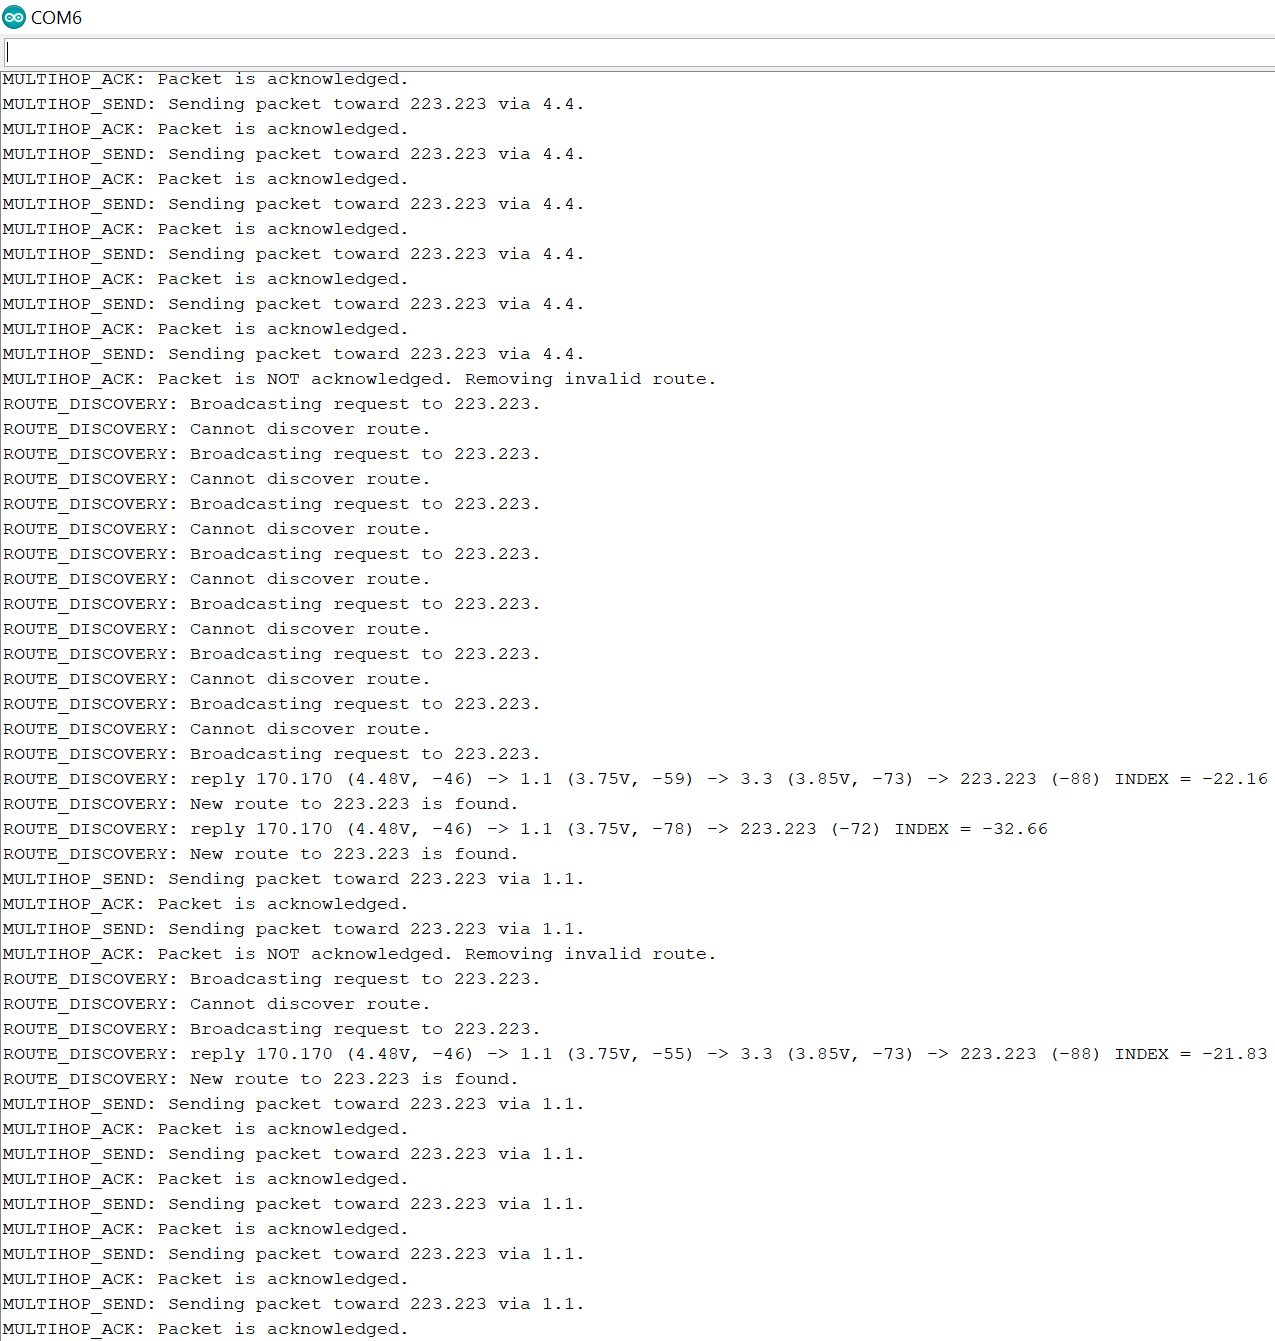
\includegraphics[width=0.7\textwidth]{test-4-source}
\caption{Output from the Source Device After Changes of Intermediate Nodes in the Network.}
\label{fig:test-4-source}
\end{figure}


After a few trials, the source learns a stable route towards the destination through the first intermediate node (1:1) and later the third intermediate node (3:3).
It sends data packets to and receives acknowledgements from the destination regularly.

Figure \ref{fig:test-4-dest} shows the output from the destination device.
It first receives sensors reading from the source through the fourth intermediate node (4:4). 

\begin{figure}
\centering
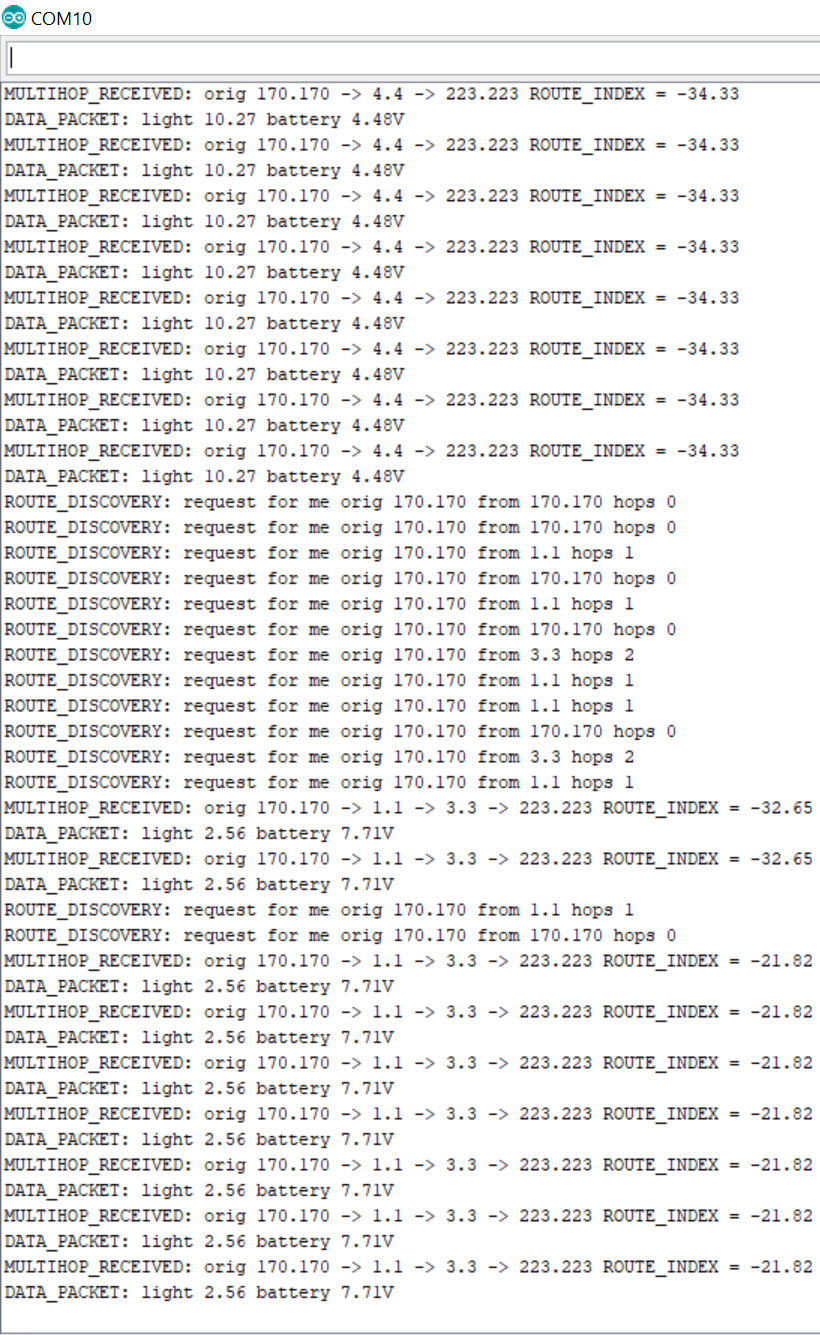
\includegraphics[width=0.7\textwidth]{test-4-dest}
\caption{Output from the Destination Device After Changes of Intermediate Nodes in the Network.}
\label{fig:test-4-dest}
\end{figure}

After the fourth node is switched off, it receives several RREQ from the source when the source is requesting a route to it.
After the source learns a stable route towards the destination, the destination device starts regularly receiving data packets from the source device through the new route.
The new route goes through the first intermediate node (1:1) and later the third intermediate node (3:3).

\section{Extra Testing: Network Performance Test}

The overall wireless network performance can be spited into several parts.

\subsection{Network Stability}

First, we use the data packet loss rate as the network stability standard. Because that transmitted data is easily interference by the other raido-wave signals. The network performance is also influenced by that item.

In this section, the data packet loss rate is the main parameters that should be given attention.

We implemented two different kinds of protocol and tested them under 3 different circumstances. The result of this part is shown in Figure \ref{fig:packetloss} and \ref{fig:packetlossnew}.

\begin{figure}
    \centering
    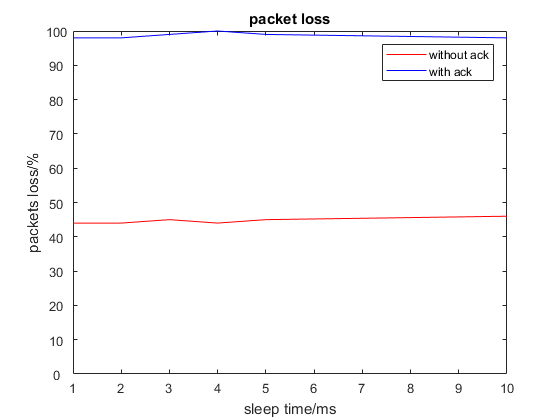
\includegraphics{Figures/packetloss.png}
    \caption{Test packet loss rate}
    \label{fig:packetloss}
\end{figure}

\begin{figure}
    \centering
    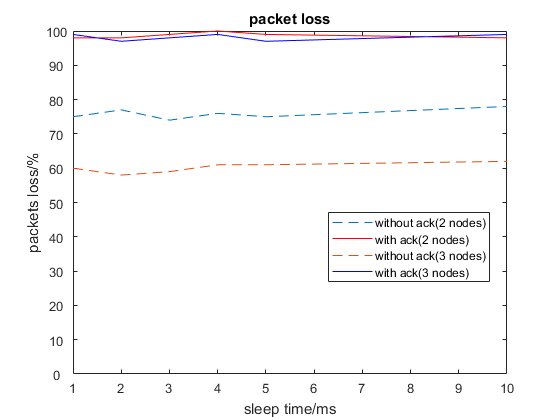
\includegraphics{Figures/packetlossNEW.png}
    \caption{Test packet loss rate}
    \label{fig:packetlossnew}
\end{figure}

\subsection{Network Data Sending Rate}

Second, we need to know the maximum packet process rate of the network using different routing algorithms.

In this section, we separate the test procedure into 2 parts. The first part is aimed to test the performance of different algorithms, the second part is aimed to test the maximum performance on the proposed AODV algorithm. Also, in AODV algorithm, we implemented 2 different method, the first method is standard AODV, which dose not use ACK packet. The second method is modified AODV, which will use ACK packet to reduce packet loss and improve the performance of the network.

\subsection{Performance Comparison of Different Algorithms}

In this part, we adopted three different index algorithms to test the performance of the wireless network.
The first algorithm is proposed index Formula \ref{equ:index3}.

\begin{equation}
    \text{Route Index} = 
    \frac{\sum_i^N{RSSI_i}}{N \times H}
\label{equ:index3}
\end{equation}

The second algorithm is route choose directly using hops, can be represented as Formula \ref{equ:index1}.

\begin{equation}
    \text{Route Index} = H
\label{equ:index1}
\end{equation}

The final one is proposed using both RSSI and HOPS as presented as Formula \ref{equ:index2}.

\begin{equation}
    \text{Route Index} = 
    {\sum_i^N{RSSI_i}}
\label{equ:index2}
\end{equation}

During the test procedure, we found that these 3 algorithms has no big influence on  the performance of the internet. Results can be seen in \ref{fig:algorithm_comp}. 

\begin{figure}
    \centering
    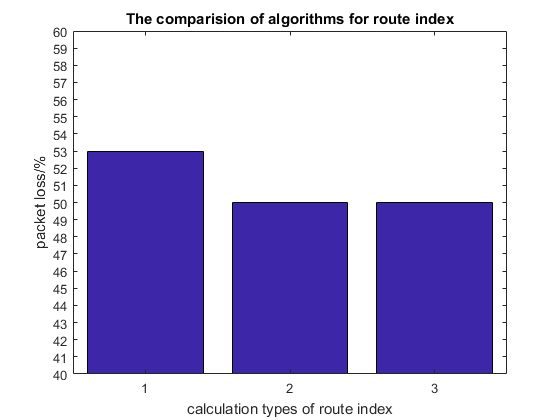
\includegraphics{Figures/algorithm.png}
    \caption{Comparison of different algorithms on the performance of the Network}
    \label{fig:algorithm_comp}
\end{figure}

As can be seen, the difference of 3 different algorithms is within the normal data variance range. Thus, routing algorithms tested in the test environment.
The reason for this is that under the circumstance of the test environment, all routes is not stable. Even if the algorithm choose the right path at the stage of building the data path, the result is still not stable.

\subsection{Maximum Data Sending Rate on Proposed Algorithm}

In this part, different sleep time is tested to find the maximum data processing rate of the Sensinode. Experiment method is the same as explained before. We use two Sensinode using multicast method. The different sleep will denote different data sending rate, as calculated using Formula \ref{equ:speed}. 

\begin{equation}
    \text{Send speed} = 
     \frac{\text{unit time}}{\text{sleep time} + \text{processing time}}
\label{equ:speed}
\end{equation}

The result of the test is shown in \ref{fig:processability}

\begin{figure}
    \centering
    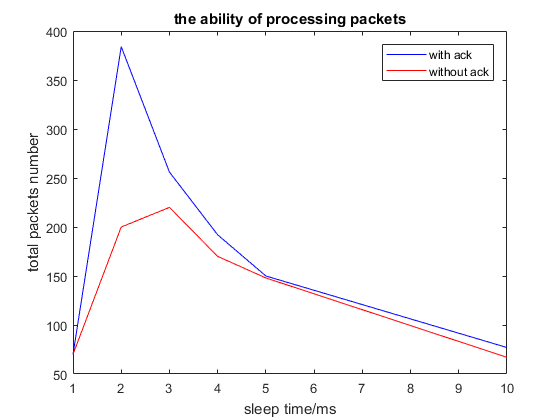
\includegraphics{Figures/processability.png}
    \caption{Process speed of the network}
    \label{fig:processability}
\end{figure}

From the result, we could calculate that the data sending rate a Sensinode could handle is approximate 8kbit/s. The condition of generating that data rate is we use a 112-bit-length packet each time, and we could send approximate 70 packets every second. The sending rate could not be higher, due to higher sending rate will cause the Sensinode restart due to massive unprocessed data packets.

\chapter{Discussion}
\label{chap:discussion}


\section{Conclusions}
TODO...

\section{Further Work}


After examining the performance of the network. We found that there exists severe packet loss when data sending rate is high. There are several causes could lead to such result. Further work should focus on resolving this problem.

In the coursework requirement, there is no need for data acknowledgement. In such circumstance, the sender won’t know whether the data packet is successfully sent. Thus, we could add data acknowledgement in the process of sending data. After add data acknowledgement, the data sending rate is limited, due to that we could only send one packet at each time before data acknowledgement is received.

Thus, another improvement area is adding data sending buffer. When handling data buffer, we could add both data sending buffer and data receiver buffer. The advantage of adding sending buffer is that we could send more data at each time. As a result, the throughput of the network is increased. The advantage of adding receiving data buffer is that when receiving data packet which has no route to be sent, we could store the data in the buffer and wait for the correct route is found. In this way, less data packets are dropped when the topology of the network is changed.

Also, the AODV protocol we implemented in the coursework is not standard protocol. We could also implement some extra features required by AODV protocol. Such as RRER reply mechanism and data queuing strategy.

In conclusion, further is focused on improving the data throughput performance of the network.








% Include a Chapter names References to the table of content
\addcontentsline{toc}{chapter}{References}
% Rename Bibliography to References
\renewcommand\bibname{References}
\bibliography{Bib/tex}

% Include authors publications and appendix section
% \addcontentsline{toc}{chapter}{Publications}
\chapter*{Publications}
\label{chap:Publications}

% Author publication section
% If not using the references per chapter option you need to include the bibliography inline
% This was done by creating a bibtex file containing the publications and including in a separate LaTeX file, using \nocite{*} this includes all bibtex items, generating the .bbl file and then copying and pasting below.

List of authors academic publications

\begingroup
% Remove title and space of header for this chapter
\titleformat{\chapter}[display]
    {\normalfont\huge\bfseries}{\chaptertitlename\ \thechapter}{20pt}{\Huge}
\titlespacing*{\chapter}{0pt}{0pt}{-80pt}
\renewcommand\bibname{}
\begin{thebibliography}{1}

%\bibitem{}

\end{thebibliography}
\endgroup

% To include copies of the publications use the includepdf package and point to .pdf files of papers
% Example
%\includepdf[pages=-, pagecommand=, templatesize={5in}{10in}]{Publications/Pubs/le1_biothreads.pdf}

% % Appedix
\appendix

\begingroup

\chapter{Source Code}
\label{app:code}


\endgroup


\end{document}
